\documentclass{amsart}
\usepackage{graphicx}
\usepackage[margin=2.5cm]{geometry}
\usepackage{multicol}
\usepackage{amsmath}
\usepackage{caption}
\usepackage{algorithm}
\usepackage{algorithmicx}
\usepackage{algpseudocode}
\usepackage{mathrsfs}
\usepackage{float}
\usepackage{xcolor}
\usepackage{subfigure}
% Para tablas:
\usepackage{booktabs}
\usepackage{multirow}

% Para incluir números de línea que faciliten la revisión
%\usepackage{lineno}
%\linenumbers

% Para hipervínculos:
\usepackage{hyperref}
\hypersetup{
    colorlinks=true,
    linkcolor=magenta,
    filecolor=magenta,      
    urlcolor=black,
    pdftitle={Reforestation Logistic Transport Optimization},
    pdfpagemode=FullScreen,
    citecolor = blue
    }
\urlstyle{same}
\usepackage[english]{babel}
\usepackage[babel]{csquotes}
\usepackage[backend=biber, style=apa]{biblatex}
\DeclareLanguageMapping{english}{english-apa}
\bibliography{Sources/referencias.bib}

\newenvironment{Figura}
{\par\medskip\noindent\minipage{\linewidth}}
{\endminipage\par\medskip}


\begin{document}

% ------------------------------- PORTADA -----------------------------
    \begin{center}
        {\bfseries\LARGE Tecnol\'ogico de Monterrey\par}
        {\scshape\Large Escuela de Ingenier\'ia y Ciencias\par}
        \vspace{0.5cm}
        %{\scshape\Huge Logísticas Verdes: Optimización de Rutas de Trasnporte en Reforestación \par}
        {\scshape\Huge Green Logistics: Transport Routing Optimization for Reforestation\par}
        \vspace{0.5cm}
        %{\small Author 1 \hspace{5pt} Author 2\hspace{5pt} Author 3 \par Author 4 \hspace{5pt} Author 5\par}
    
        {\small Juan Jos\'e H. Beltr\'an \textsuperscript{1} \hspace{5pt} Kevin Mart\'inez-Trinidad \textsuperscript{2} \hspace{5pt} Ricardo Kaleb Flores-Alfonso \textsuperscript{3} \par Jes\'us Ramirez-Mendieta \textsuperscript{4} \hspace{5pt} Fernando Elizalde-Ram\'irez \textsuperscript{5}\par}
        
        \vspace{0.5cm}
        
        {\tiny \textsuperscript{1} juanjobelt@outlook.com \hspace{3pt} \textsuperscript{2} kevinjtrinidad@gmail.com \hspace{3pt}  \textsuperscript{3} r.kaleb@hotmail.com \hspace{3pt} \textsuperscript{4} Jesusramirezm04@hotmail.com \hspace{3pt} \textsuperscript{5} fer\_elizalde@tec.mx \par}
        
        
        
        %\begin{table}[h]
        %    \begin{tabular}{cccc}
        %    \begin{tabular}[c]{@{}c@{}}Author 1\\ a00836747@tec.mx\end{tabular} &
        %        \begin{tabular}[c]{@{}c@{}}Author 2\\ a@tec.mx\end{tabular} &
        %        \begin{tabular}[c]{@{}c@{}}Author 3\\ a@tec.mx\end{tabular} &
        %        \begin{tabular}[c]{@{}c@{}}Author 4\\ a@tec.mx\end{tabular}
        %    \end{tabular}
        %\end{table}
        \vspace{0.3cm}
        {\small \today}
        \vspace{0.5cm}
        
        \rule{16.5cm}{0.1pt}
    \end{center}


% -----------------------------Abstract---------------------------------

\section*{Abstract}
    This paper addresses the optimization of transport logistics in reforestation projects, focusing on minimizing time and costs associated with plant deliveries. A Vehicle Routing Problem (VRP) framework was applied, using mixed-integer linear programming to determine optimal delivery truck routes while considering vehicle capacities and delivery demands. Additionally, a heuristic solution was implemented to reduce computational time while maintaining near-optimal results. Based on data from a reforestation entity in Mexico, findings demonstrate that the heuristic model efficiently manages reforestation logistics.
    
{\subsection*{Keywords} Optimization, vehicle routing problem, linear programming, heuristics, logistics, reforestation.}


% -----------------------------Introduction---------------------------------

    \section{Introduction}
        Climate change and droughts pose significant challenges to ecosystems and human activities. Deforestation is a major contributor to these issues, accelerating climate change and reducing water availability. In Mexico, deforestation remains a critical problem, often occurring illegally or irresponsibly \parencite{WRI2023}. Reforestation programs help mitigate these negative effects, yet they operate with limited resources and must be completed within a short time frame each year.

         Consequently, optimizing transport routes and scheduling is essential to reduce costs and improve efficiency in reforestation logistics, and increase as much as possible the probabilities of successfully completing the project, using the least amount of resources possible.
         
         The Vehicle Routing Problem (VRP) is a well-researched combinatioral optimization problem with significant industrial applications. It involves determining a set of routes for a fleet of vehicles departing from one or more depots to satisfy the demand of geographically dispersed customers \parencite{Sarmiento2014}.
         
         Previous studies have applied VRP models to reforestation logistics, such as \cite{VRPReforestation}, wich explores visiting different forest areas for resource assessments but ultimately resorted to a case study due to computational complexity. 
         
         Furthermore, other transportation and distribution logistic cases have been explored. \cite{Nurprihatin2021} which optimized rice distribution using Monte Carlo simulations and genetic algorithms, staying with a two-steps linear programming method, a transportation model followed by a Capacitated Vehicle Routing Problem. The study considers other transportation methods like ships and planes and designs a conditional methodology combining the steps mentioned before. Meanwhile, \cite{Khan2014} models a mosquito coil distribution as an assignment problem, considering multiple clients and 3 warehouses. In \cite{Feillet2014}, a multiday VRP based on time-classes is introduced to address a problem of transportation of people with disabilities, where each customer is served almost daily with some consistency being expected in the service, the solution is found using a large neighborhood search heuristic, with each iteration solving a complex VRP with multiple time windows and no waiting time.
      
        This paper aims is to minimize both distance and time in transporting plants to reforestation sites. To do this, it is proposed to build an optimized work plan that orders routes to ensure efficient deliveries.
        



% --------------------------- Materials and Methods ---------------------------------

\section{Materials and Methods}
    \subsection{Problem Description}
    Is the intention, through a mathematical model and/or a heuristic algorithm, to provide a method to optimally plan the routes necessary to comply the number of individuals that will be necessary for each section of the reforestation land (Figure \ref{fig:tablaDePoligonos}). The partnered entity has established specific planting requirements (Available on the \underline{\href{https://github.com/JuanjoBelt/VRP-ReforestationTransportLogistics}{GitHub repository}}), which are identical for each hectare to be reforested. These requirements are scaled, maintaining their proportions between species when dealing with fractions of hectares.
    
    The problem closely resembles a VRP with split deliveries, where a single depot supplies multiple locations using vehicles with identical or varying capacities \parencite{Dror}.
    
    Given the lack of detailed path information, Euclidean distances were used as cost metrics. Since the number of vehicles available is not known, it was decided to set the number of vehicles as the minimum required cycles to meet all the demands, with each cycle beginning and ending at the depot. 

    To obtain the distances between the nodes, the image with the geographic location of the polygons (Figure \ref{fig:tablaDePoligonos}) was used, considering the scale in meters presented. A Python code was implemented allowing to obtain the distance between each node by simply entering the approximate coordinate of the centroid of each one.
        
        \begin{figure}[ht]
            \centering
            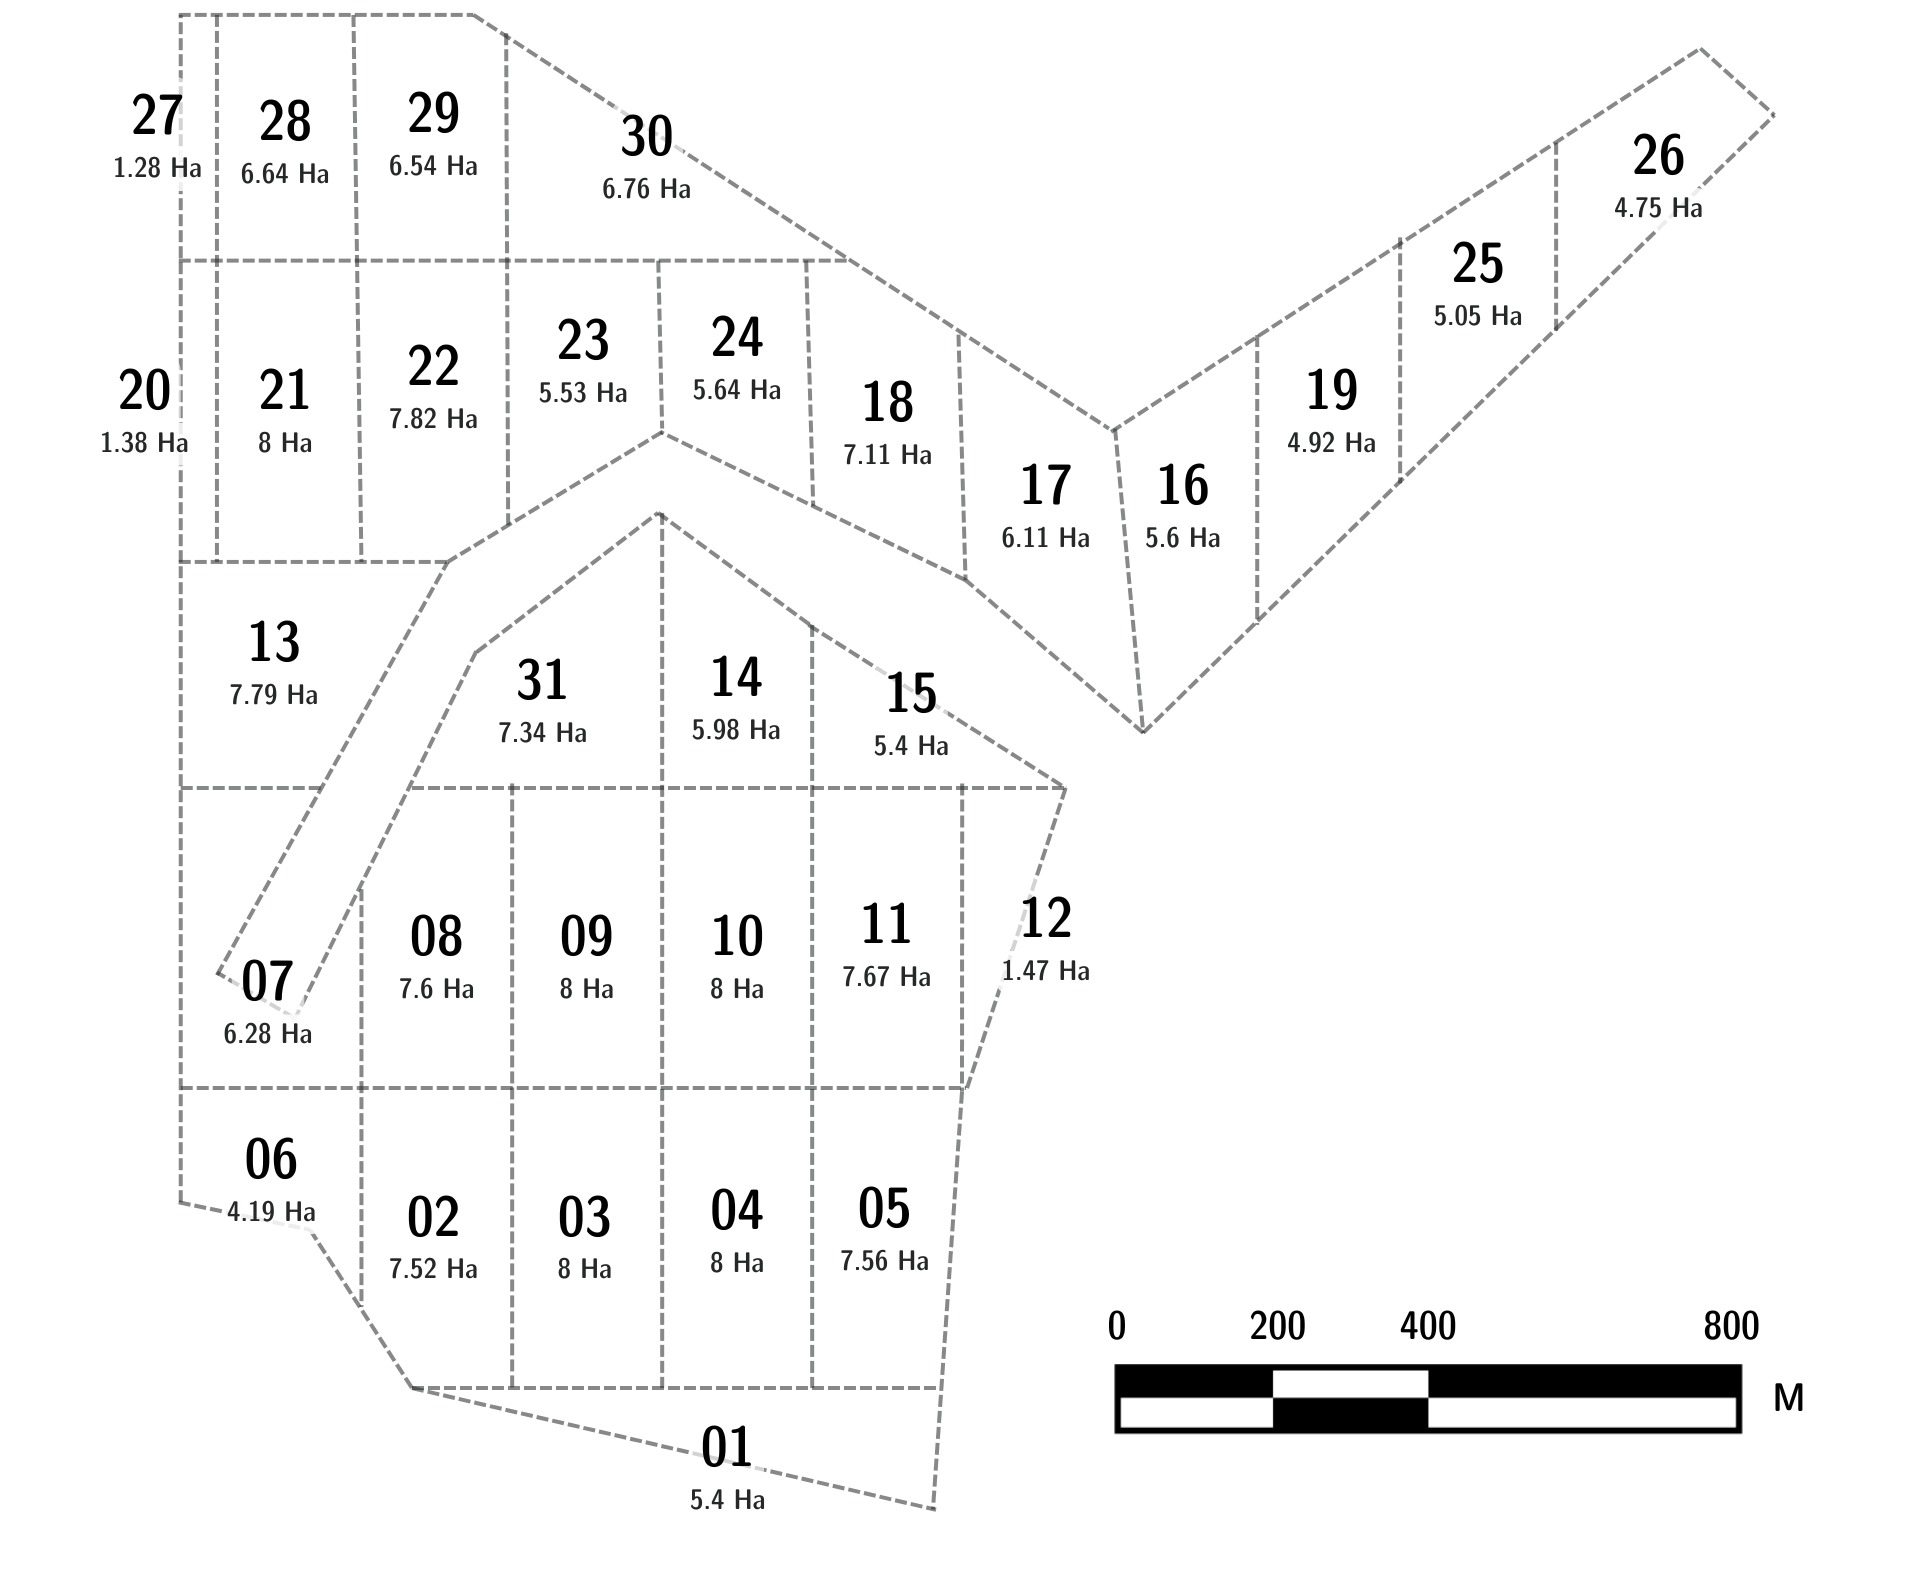
\includegraphics[width=0.5\linewidth]{Sources/Field.png}
            \caption{Sections of land to be reforested. Its numbering and area in hectares are shown.}
            \label{fig:tablaDePoligonos}
        \end{figure}
    
    \subsubsection{Considered parameters}
    
    The following values for the parameters were obtained from the partnered reforestation entity.
    
    \begin{itemize}
        \item \textit{Average speed of vehicles:} 20 km/h. Considering heavy-duty trucks, these tend to have low acceleration and speed, mainly when dealing with unpaved roads.
        \item \textit{Vehicle capacity:} 1 hectare per trip. All vehicles are considered to have identical capacity, as we are actually considering a single vehicle that makes the routes consecutively.
        \item \textit{Node demands:} determined by the area in hectares for each polygon.
        \item \textit{Loading and unloading time:} 30 minutes per hectare.
        \item \textit{Distance between nodes:} Euclidean distances between polygon centroids.
        \item \textit{Working day length:} 8 hours (the standard in Mexico).
    \end{itemize}
    
    %Since the aim is to optimize the time it takes for the vehicles to supply the requested demands, it is necessary to consider the speed at which these vehicles move. Being heavy-duty trucks, these tend to have low acceleration and speed, mainly when dealing with unpaved roads, as in this case study. We consider an average speed of 20 km/h, since there are no established roads on most of the routes and the reforestation area has a uniform altitude.
    
    \subsubsection{Model Assumptions and Limitations}
        The assumptions of the model and the limitations they cause in it are stated below, as well as possible solutions for further works.
        
        \begin{itemize}
            \item \textit{Euclidean Distance Approximation:} Since the Euclidean distance between nodes is considered, it is ignored that this metric will become misleading once some hectares begin to be reforested, since it will be impossible to cross them on the route. A possible solution would be to consider dynamic distances according to the reforested spaces; or directly consider static distances corresponding to routes that are always guaranteed to be available. In this last case the modification would only be a change of values in the parameters.
            \item \textit{Fixed Load Distribution:} The way the load is distributed in the vehicles is not subject to modification, since it is assumed that they are always loaded with the species and specimens necessary to reforest exactly one hectare. Therefore, it cannot be ruled out that there is a better solution by altering this method.
        \end{itemize}
    
    
    \subsubsection{Problem Simplification}
    
    Note that by assuming identical vehicle capacities (as it happens in this case), many of the nodes need one or more fully loaded trucks, that is, it is necessary to make multiple routes where the vehicles leaves the origin node, arrives at the node to be supplied, unloads all the cargo it carries and returns to the origin node, since it can be proven that these routes are part of the optimal solution. Considering this, most of the delivery cycles can be easily determined just as $\lfloor\frac{\text{\textit{Node demand}}}{\text{\textit{Tuck capacity}}}\rfloor$, leaving only a demand of $\left( \text{\textit{Node demand}} \mod \text{\textit{Truck capacity}} \right)$ to be covered.
    
    For example, in this context, if a node has a demand of 6.28 ha and the vehicles capacity is 1 ha, the model will always carry 6 fully loaded trucks, leaving the node with only the \textit{decimal part} to supply. The order in which these routes are executed does not change the cost and calculating the latter does not require great computational capacity.

    It can then be seen that the problem is reduced to determining the routes to follow to supply the \textit{decimal parts} of the demands, thus reducing the complexity of the problem. For this simplified model it can be observed that the number of nodes is reduced to 26, since there are 5 that have integer demands.

    An exact solution was initially attempted using mixed-integer linear programming (See Section \ref{ModeloMatematico}). This model was implemented in GAMS modeling software with CPLEX solver and Python using PuLP library with a Gurobi solver. However, the proposed model is too complex for the educational license in GAMS, while in Python, the model takes an inadmissible amount of time. Instead we use it to prove the heuristic solution in smaller problems. This can allow us to compare the optimal solution and the heuristic proposed.

        The following heuristic solution is proposed (See Section \ref{MetodoHeuristico}), which, through Python code, allows obtaining a very close solution to the optimal one, using much less memory and execution time.
        
        

    \subsection{Mathematical Model}\label{ModeloMatematico}
        \subsubsection{Sets} 
        
        
        Set $N=\{1, 2, ... , n\}$ represents the clients (demanding nodes). It is defined $V=N \cup \{0\}$, where $0$ represents the depot. $A$ is the set of arches that join the elements in $V$. $A'$ is the set of arches that join the elements of $N$. With the above, $G=(V, A)$ is a directed and complete graph of nodes $V$q and edges $A$. It's defined $K = \{1, 2, ..., m\}$, representing the vehicles (or the different routes that must be taken).
        

        \subsubsection{Parameters}
        
        
        Let $n \in \mathbb{N}_0$ the number of customers, each with a demand of $q_i : i \in N$. Let $m \in \mathbb{N}$ the maximum number of vehicles (or independent routes) available, all of them with capacity $L \in \mathbb{R}^+$. Note that a lower bound can be placed for $m \geq (\sum q_i) \div L$. The graph $G$ has costs per unit $c_{a} : a \in A$. Let $\mathcal{M}$ a constant large enough to relate continuous and binary variables in constraints that is at least equal to the maximum demand. Let $v$ a constant corresponding to the average speed of vehicles in meters/hour, and $t$ a constant corresponding to the charging or discharging time measured in hours.


        \subsubsection{Variables}
        
        
        Let $x_{ijk}$ a binary variable that takes value $1$ if vehicle $k$ uses the edge $(i, j)$ on his route, or take value $0$ if it's not used. Similarly, $w_{ijk} \geq 0$ represents the amount of material transported by the vehicle $k$, leaving node $i$ and to deliver to the node $j$. Finally $u_{ik} \in \mathbb{Z}^+$ takes a value corresponding to the order in which the node $i$ is visited by the vehicle $k$.

        
        \vspace{0.4cm} Posed as a linear programming problem, it can be written as follows:
            
            \begin{equation} \label{eq:1}
                Minimize \hspace{0.5cm} v^{-1} \sum_{i \in V} \sum_{j \in V} \sum_{k \in K} c_{ij} x_{ijk} + 2t \sum_{i \in V} \sum_{j \in V} \sum_{k \in K} w_{ijk} \hspace{0.5cm} : i \neq j
            \end{equation}

        Subject\hspace{0.07cm} to \hspace{0.5cm}
        
        \begin{equation} \label{eq:2}
            \sum_{j \in V} x_{ijk} - \sum_{j \in V} x_{jik} = 0 \hspace{0.5cm} : i \neq j \hspace{0.5cm} \forall i \in V, \hspace{0.5cm} k \in K
        \end{equation}

        
        \begin{equation} \label{eq:3}
            \sum_{j \in N} x_{0jk} = 1 \hspace{0.5cm} \forall k \in K
        \end{equation}

        
        \begin{equation} \label{eq:4}
            \sum_{i \in V} \sum_{j \in V} w_{ijk} \leq L \hspace{0.5cm} : i \neq j \hspace{0.5cm} \forall k \in K
        \end{equation}

        
        \begin{equation} \label{eq:5}
            \sum_{i \in V} \sum_{k \in K} w_{ijk} \geq q_j \hspace{0.5cm} : i \neq j \hspace{0.5cm} \forall j \in N
        \end{equation}

        
        \begin{equation} \label{eq:6}
            u_{ik} - u_{jk} + n x_{ijk} \leq n - 1 \hspace{0.5cm} : i \neq j \hspace{0.5cm} \forall i,j \in N, \hspace{0.2cm} k \in K
        \end{equation}

        
        \begin{equation} \label{eq:7}
            w_{ijk} \leq \mathcal{M} x_{ijk} \hspace{0.5cm} \forall i,j \in V, \hspace{0.2cm} k \in K
        \end{equation}

        
        \begin{equation} \label{eq:8}
            x_{ijk} \in {1, 2} \hspace{0.5cm} \forall i,j \in V, \hspace{0.2cm} k \in K
        \end{equation}

        
        \begin{equation} \label{eq:9}
            w_{ijk} \geq 0 \hspace{0.5cm} \forall i,j \in V, \hspace{0.2cm} k \in K
        \end{equation}
        
    
        
        
        \vspace{0.4cm}
        The objective function to be minimized (Equation \ref{eq:1}) is the sum of the product of the costs per arch and the binary that indicates whether it was used or not, multiplied by the reciprocal of the speed, all of this representing the time invested in traveling distances; plus the sum of all the loads delivered multiplied by $2t$, which is the loading/unloading time, which is assumed to vary linearly depending on the number of plants to be unloaded. 
        
        
        Equation \ref{eq:2} corresponds to the first group of constraints, which conserves the flow of vehicles. Equation \ref{eq:3} ensures that all cars visit node zero (depot). Constraints represented by Equation \ref{eq:4} corresponds to the maximum load of each vehicle. Equation \ref{eq:5} is to satisfy the demands of each customer. Equation \ref{eq:6} aim to avoid subtours, by assigning each node a positive integer corresponding to the order in which they are visited by each vehicle. Finaly, Equation \ref{eq:7}, Equation \ref{eq:8} and Equation \ref{eq:9} are about the nature of the variables: $x_{ijk}$ must equal zero only if $w_{ijk}$ is equal to $0$, and must be equal to $1$ otherwise. $x_{ijk}$ is a binary variable. $w_{ijk}$ must be greater than or equal to zero to avoid transporting a negative amount of material (plants).

        \subsection{Heuristic Approach}\label{MetodoHeuristico}
        A greedy heuristic algorithm was chosen, which starts by completely supplying the demand of the node furthest from the depot, and then unloads the remaining resource at the node closest to the one previously visited. This makes deliveries more efficient, since the furthest customers generate most of the costs, this algorithm allows us to reduce the number of times it is necessary to travel to a distant node. A pseudocode can be seen in Algorithm \ref{Pseudocode Heuristic}.
        
                \begin{algorithm}
    \caption{Greedy Heuristic for Demand Fulfillment}
    \begin{algorithmic}[1] 
        \State Sort nodes by distance from the depot in descending order
        \State Initialize vehicle at depot with full capacity $L$
        
        \While {there are unsupplied customers}
            \State Select and move to farthest unsupplied node $i$ from the depot
            \State Supply all the possible demand in $i$
            \State Update remaining capacity
            \If {remaining capacity $>$ 0}
                \State Select and move to nearest unsupplied node from the node $i$
                \State Supply all the possible demand in closest node
                \State Update remaining vehicle capacity
            \Else
                \State Return to depot to reload
            \EndIf
        \EndWhile
        
        \State Return to depot
    \end{algorithmic}
\label{Pseudocode Heuristic} 
\end{algorithm}
            
        
        \subsection{Scheduling Optimization}\label{OrderRoutes}
        Having obtained the optimal routes, it is important to make a plan, such that the number of working days required is minimized. Assuming that a route cannot be interrupted once it is started, the routes are completely independent of each other and can be reordered at will. The following mathematical model is proposed:
        
        Let $h$ be the hours available for tours per day. Set $M=\{1, 2, ... , m\}$ represents the days on which the routes will be distributed. Set $N = \{1, 2, ..., n\}$ represents the routes to be distributed. Each route has an associated cost $c_i$, which is the time it takes to travel the route $i \in N$ distributing the truck's load. Let $x_{ij}$ be binary variables, which take the value of 1 if the route $i\in N$ will be done in the day $j \in M$; and let $d_j$ be binary variables, which take the value of 1 if at least one route is programmed to be done on the day $j \in M$, or 0 otherwise.
        
        Posed as a linear programming problem, it can be written as follows:
        
        \begin{equation} \label{eq:10}
            Minimize \hspace{0.2cm} \sum_{j \in M} d_j
        \end{equation}
        
        Subject \hspace{0.07cm} to \hspace{0.2cm} 
        
        \begin{equation} \label{eq:11}
            \sum_{i \in N} c_i*x_{ij} \leq h * d_j \hspace{0.5cm} \forall j \in M
        \end{equation}

        \begin{equation} \label{eq:12}
            \sum_{j \in M} x_{ij} = 1 \hspace{0.5cm} \forall i
        \end{equation}
        
        Where Equation \ref{eq:10} aims to minimize the number of days required to complete the plan. Meanwhile, Equation \ref{eq:11} restricts the model so the total time made by the routes on a day is not superior to the working hours available on the same day and Equation \ref{eq:12} ensures that all the routes are completed.


        
        By solving this model, considering an 8-hour work day, the configuration that minimizes the number of days required to complete the distribution of plants to all polygons can be found.

% -------------------------------------- Experimental Results--------------------------------------
    \section{Experimental Results}
        \subsection{Solutions with Small Cases}\label{SolutionsWithSmallCases}
        To validate the heuristic approach, three problem sizes (5, 10 and 12 nodes) were tested against exact solutions. These were tested in 5 samples took randomly (See Table \ref{tab:5,10,12nodos}). GAP is the standard: percentage distance from optimum, considering the complete problem solution: integer part plus decimal part, which is the reference that is significant for reforestation programs. In order to guarantee the equality of conditions between our samples, no other zero demand nodes besides of the base were included. Likewise, in Table \ref{tab:TiemposDeComputo} , the heuristic model's solutions were within 5\% of optimal results while significantly reducing processing time.
        
        \begin{table}[h!]
                \scriptsize
                \begin{tabular}{llrrrrrr}
                \toprule
                \multicolumn{1}{c}{\textbf{\#}} &
                  \multicolumn{1}{c}{\textbf{Sample Nodes}} &
                  \multicolumn{1}{c}{\textbf{\begin{tabular}[c]{@{}c@{}}Optimum\\ (M.M.)\end{tabular}}} &
                  \multicolumn{1}{c}{\textbf{\begin{tabular}[c]{@{}c@{}}Time\\ (M.M.)\end{tabular}}} &
                  \multicolumn{1}{c}{\textbf{\begin{tabular}[c]{@{}c@{}}Solution\\ (H.M.)\end{tabular}}} &
                  \multicolumn{1}{c}{\textbf{\begin{tabular}[c]{@{}c@{}}Time\\ (H.M.)\end{tabular}}} &
                  \multicolumn{1}{c}{\textbf{\begin{tabular}[c]{@{}c@{}}Integer\\ Part\end{tabular}}} &
                  \multicolumn{1}{c}{\textbf{GAP}} \\
                \midrule
                1 & \{1, 18, 20, 23, 26\} & 2.33 & 0.05 s & 2.483 & 0.004 s & 16.433 & 0.81\% \\
                2 & \{1, 7, 11, 18, 20\}  & 1.97 & 0.05 s & 2.112 & 0.007 s & 21.245 & 0.61\% \\
                3 & \{1, 2, 8, 16, 18\}   & 2.40 & 0.6 s  & 2.547 & 0.003 s & 26.481 & 0.50\% \\
                4 & \{5, 17, 18, 19, 29\} & 2.33 & 0.1 s  & 2.352 & 0.003 s & 24.83  & 0.08\% \\
                5 & \{6, 7, 13, 18, 30\}  & 1.41 & 0.1 s  & 2.414 & 0.006 s & 25.094 & 3.78\% \\
                \\
                1 & \begin{tabular}[c]{@{}l@{}}\{2, 8, 13, 16, 17, 18, 20, 22, 28, 29\}\end{tabular} & 5.67 & 233 s & 5.73  & 0.032 s & 56.021 & 0.09\% \\
                2 & \begin{tabular}[c]{@{}l@{}}\{5, 8, 12, 16, 18, 19, 20, 22, 28, 29\}\end{tabular} & 6.00 & 15 s  & 6.049 & 0.005 s & 47.488 & 0.09\% \\
                3 & \begin{tabular}[c]{@{}l@{}}\{2, 5, 6, 7, 11, 17, 18, 20, 22, 30\}\end{tabular}   & 4.69 & 5.8 s & 4.734 & 0.036 s & 55.326 & 0.07\% \\
                4 & \begin{tabular}[c]{@{}l@{}}\{2, 8, 11, 18, 19, 20, 23, 26, 29, 30\}\end{tabular} & 6.14 & 3.9 s & 6.203 & 0.031 s & 50.758 & 0.11\% \\
                5 & \begin{tabular}[c]{@{}l@{}}\{2, 7, 11, 18, 19, 20, 23, 26, 29, 30\}\end{tabular} & 5.81 & 4.7 s & 5.864 & 0.012 s & 49.773 & 0.09\% \\ 
                \\
                1 & \{1, 2, 6, 8, 11, 15, 18, 19, 20, 22, 23, 29\} & 7.07 & 63 s & 7.237 & 0.027 s & 62.879 & 0.23\% \\
                2 & \{1, 2, 5, 6, 8, 15, 18, 20, 22, 25, 27, 30\}  & 6.07 & 425 s & 6.763 & 0.010 s & 60.104 & 1.04\% \\
                3 & \{1, 5, 6, 7, 8, 11, 14, 17, 18, 19, 22, 29\}   & 6.04 & 1035 s  & 6.135 & 0.036 s & 71.469 & 0.11\% \\
                4 & \{2, 3, 7, 9, 11, 13, 18, 22, 23, 25, 29, 30\} & 6.01 & 26 s  & 6.107 & 0.010 s & 72.448  & 0.12\% \\
                5 & \{2, 5, 6, 7, 11, 14, 15, 18, 21, 24, 29, 30\}  & 6.54 & 3684 s  & 6.591 & 0.013 s & 72.448 & 0.06\% \\
                \bottomrule
                \end{tabular}
                \vspace{10pt}
                \caption{Contrast between the solutions and computation times of the mathematical model and the heuristic method in 5, 10 and 12 node test cases.} 
                \label{tab:5,10,12nodos}
            \end{table}
        
        
        
    
            
            \begin{table}[ht]
                \scriptsize
                \begin{tabular}{lrrr}
                \toprule
                \multicolumn{1}{c}{\textbf{\begin{tabular}[c]{@{}c@{}}Problem Size\\ (\# Nodes)\end{tabular}}} &
                  \multicolumn{1}{c}{\textbf{\begin{tabular}[c]{@{}c@{}}Average Computing Time\\ (Mathematical Model)\end{tabular}}} &
                  \multicolumn{1}{c}{\textbf{\begin{tabular}[c]{@{}c@{}}Average Computing Time\\ (Heuristic Model)\end{tabular}}} &
                  \multicolumn{1}{c}{\textbf{\begin{tabular}[c]{@{}c@{}}Average GAP\end{tabular}}} \\
                  \midrule
                n = 5  & 0.27 s    & 0.0046 s & 1.16\%  \\
                n = 10 & 52.48 s   & 0.0488 s & 0.045\% \\
                n = 12 & 1041.7 s  & 0.0192 s & 0.31\%  \\
                n = 31 & +24 hours & 0.005 s  & — \\ 
                \bottomrule
                \end{tabular}
                \vspace{10pt}
                \caption{Computing times for different problem sizes and different soluton methods.} \label{tab:TiemposDeComputo}
            \end{table}
            
    
            \subsection{Complete Solution}
            
            The full optimization problem involved:
        \begin{itemize}
            \item A total of 26 nodes (excluding 5 nodes which have an integer demand) and, consequently, 676 arches.
            \item A total 20670 decisión variables, taking in count 3 variables groups: 10140 binary variable $x_{ijk}$, 10140 positive variable $w_{ijk}$, and 390 positive integer variables $u_{ik}$. 
            \item A total of 707 parameters formed by 676 $c_{i,j}$, 26 $q_i$, $m$, $L$, $t$, $M$ and $V$. (See Section \ref{ModeloMatematico} for parameters definitions).
        \end{itemize}
        
            \subsubsection{Exact Solution with Mathematical Model}
            Due to computational constraints, an exact solution was infeasible, it wasn't possible to solve it to optimality in a reasonable time (less than 60 hours), therefore, the solution obtained through the heuristic method is presented, expecting good quality results as shown in Table \ref{tab:TiemposDeComputo}.
            
            \subsubsection{Heuristic Solution}
            The efficiency and near-optimality of the heuristic method (presented in Section \ref{MetodoHeuristico}) have been previously supported in Section \ref{SolutionsWithSmallCases}.
            
            In total, 15 different routes, shown in Table \ref{tab:ParteDecimal}, were needed to satisfy the demand of the decimal part of the nodes. Likewise, two of the routes of the proposed model are shown graphically (see Figure \ref{fig:RutasDeEjemplo}). The rest of the routes can be accessed in the \href{https://github.com/JuanjoBelt/VRP-ReforestationTransportLogistics/tree/5030293089820a896e177f198d9ab7f23ada59e7/Resources/RouteImages}{\underline{GitHub folder}}.
            
        \begin{table}[!htp]\centering
        \scriptsize
        \begin{tabular}{lc} \toprule
        \textbf{\#} & \textbf{Route} \\\midrule
        1 & Base → Node 1 → Node 5 → Node 11 → Base \\
        2 & Base → Node 6  → Node 2 → Node 8 → Base \\
        3 & Base → Node 7 → Node 8 → Node 14 → Node 15 → Base \\
        4 & Base → Node 26 → Node 25 → Node 19 → Base \\
        5 & Base → Node 27 → Node 28 → Node 29 → Base \\
        6 & Base → Node 20 → Node 22 → Base \\
        7 & Base → Node 13 → Node 22 → Base \\
        8 & Base → Node 29 → Node 30 → Base \\
        9 & Base → Node 11 → Node 12 → Base \\
        10 & Base → Node 19 → Node 16 → Base \\
        11 & Base → Node 22 → Node 23 → Node 24 → Base \\
        12 & Base → Node 12 → Node 31 → Node 15 → Base \\
        13 & Base → Node 30 → Node 24 → Base \\
        14 & Base → Node 16 → Node 17 → Base \\
        15 & Base → Node 15 → Base \\
        \bottomrule
        \end{tabular}
        \vspace{10pt}
        \caption{Work plan for the decimal part of the demand.}\label{tab:ParteDecimal}
    \end{table}

        \begin{figure}[h!]
            \begin{center}
                \subfigure[Route 03.]{
                    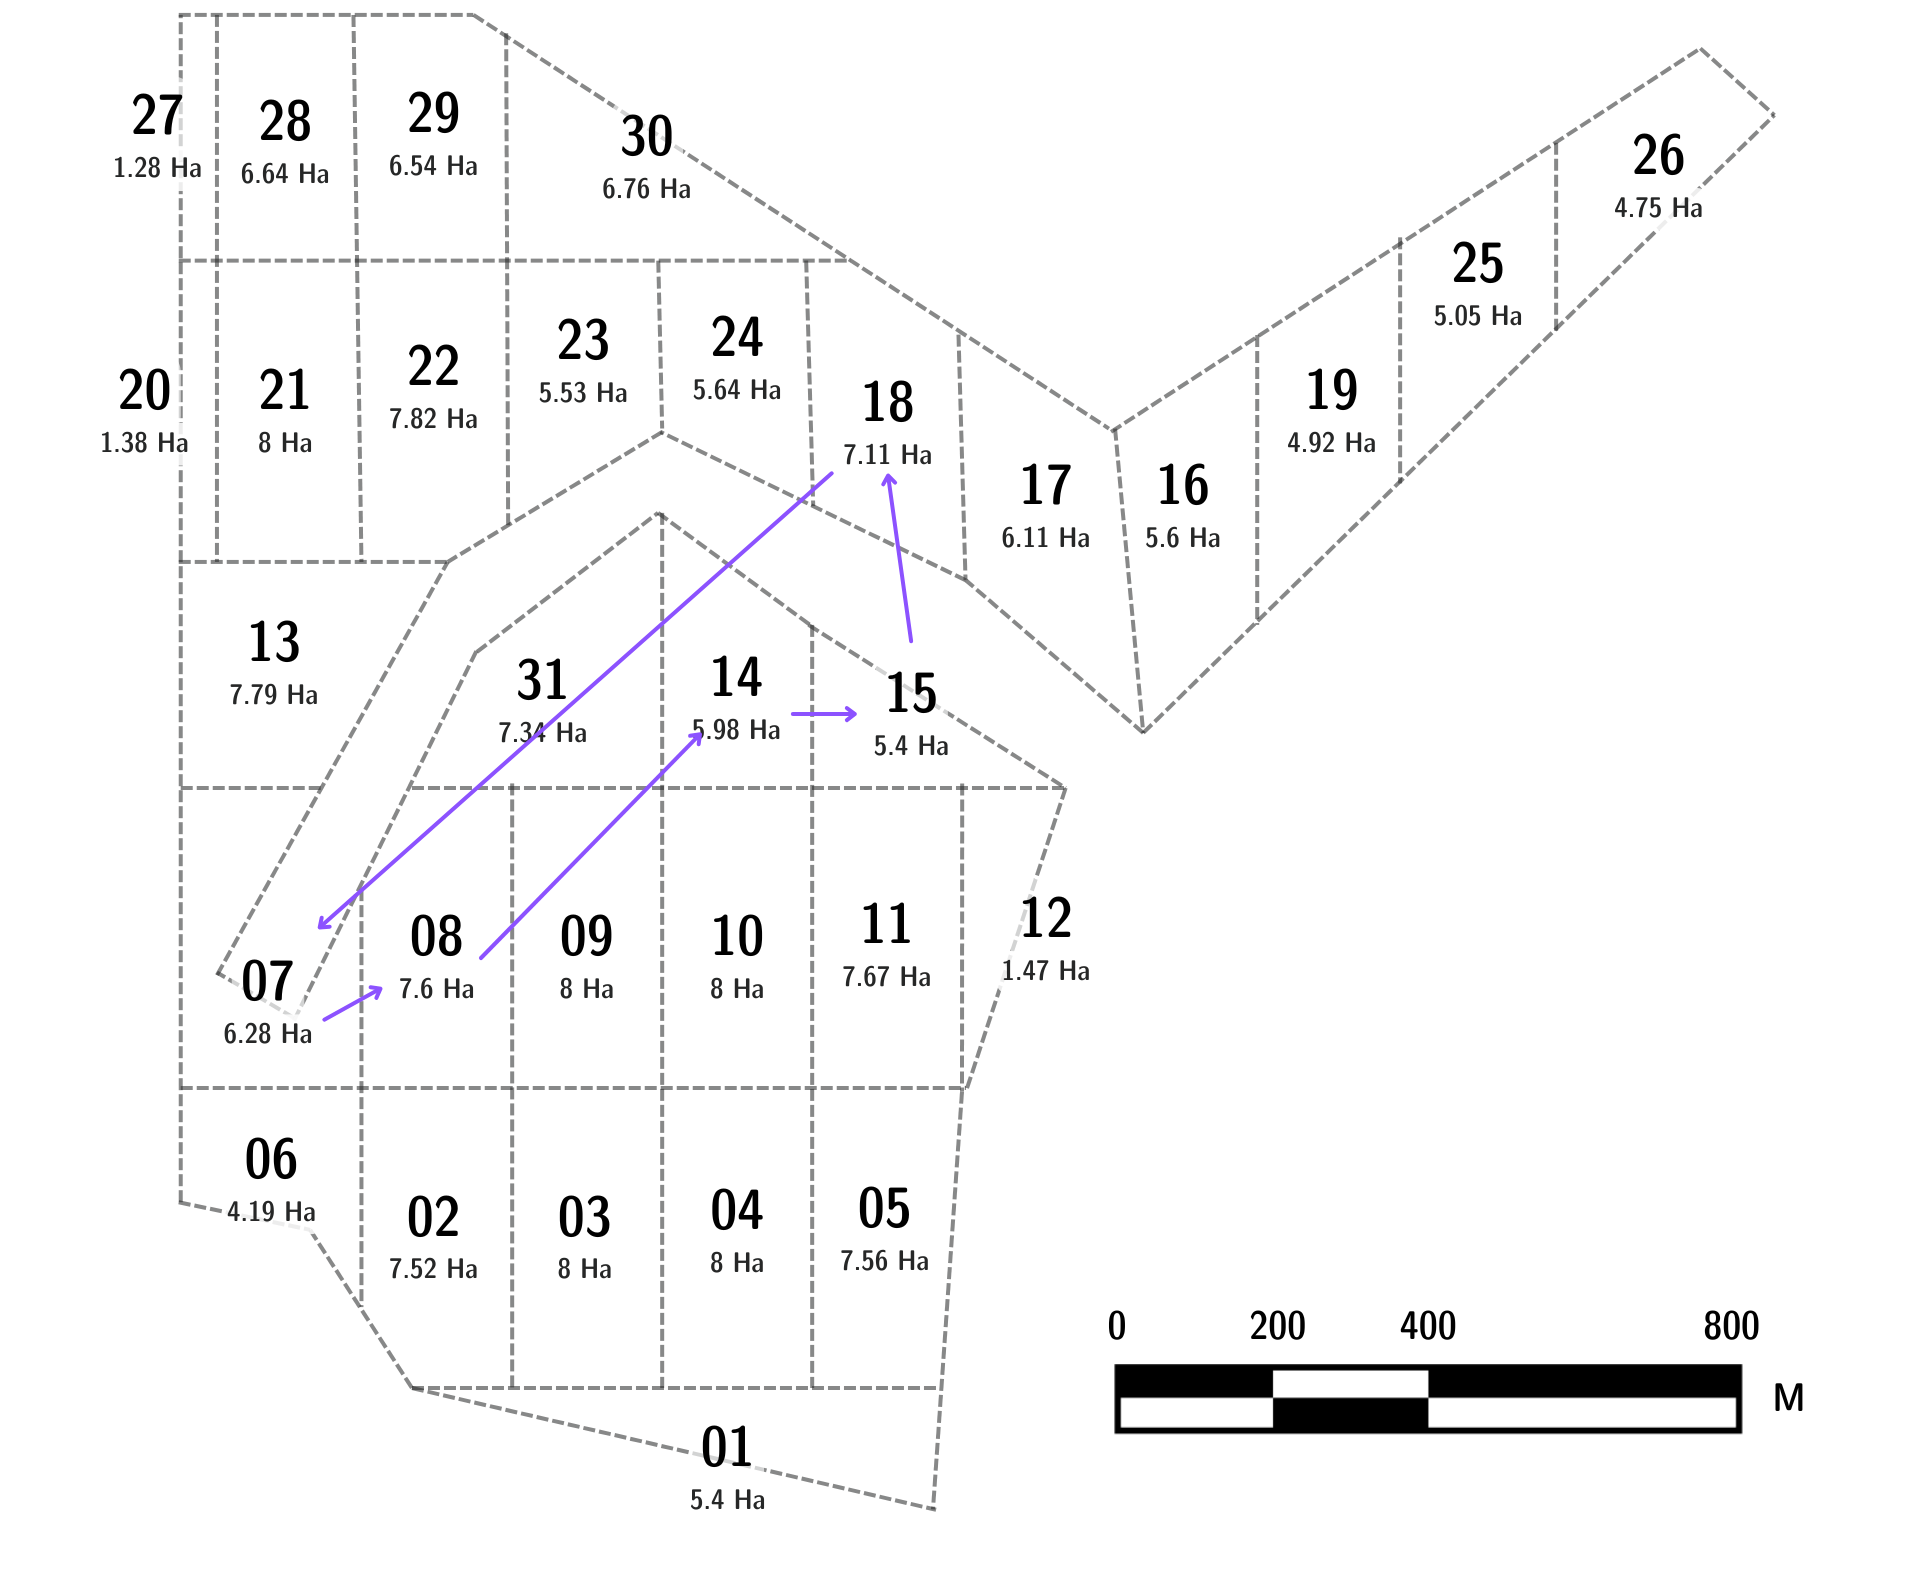
\includegraphics[width=0.40\linewidth]{Sources/Route03.png}
                }
                \subfigure[Route 13.]{
                    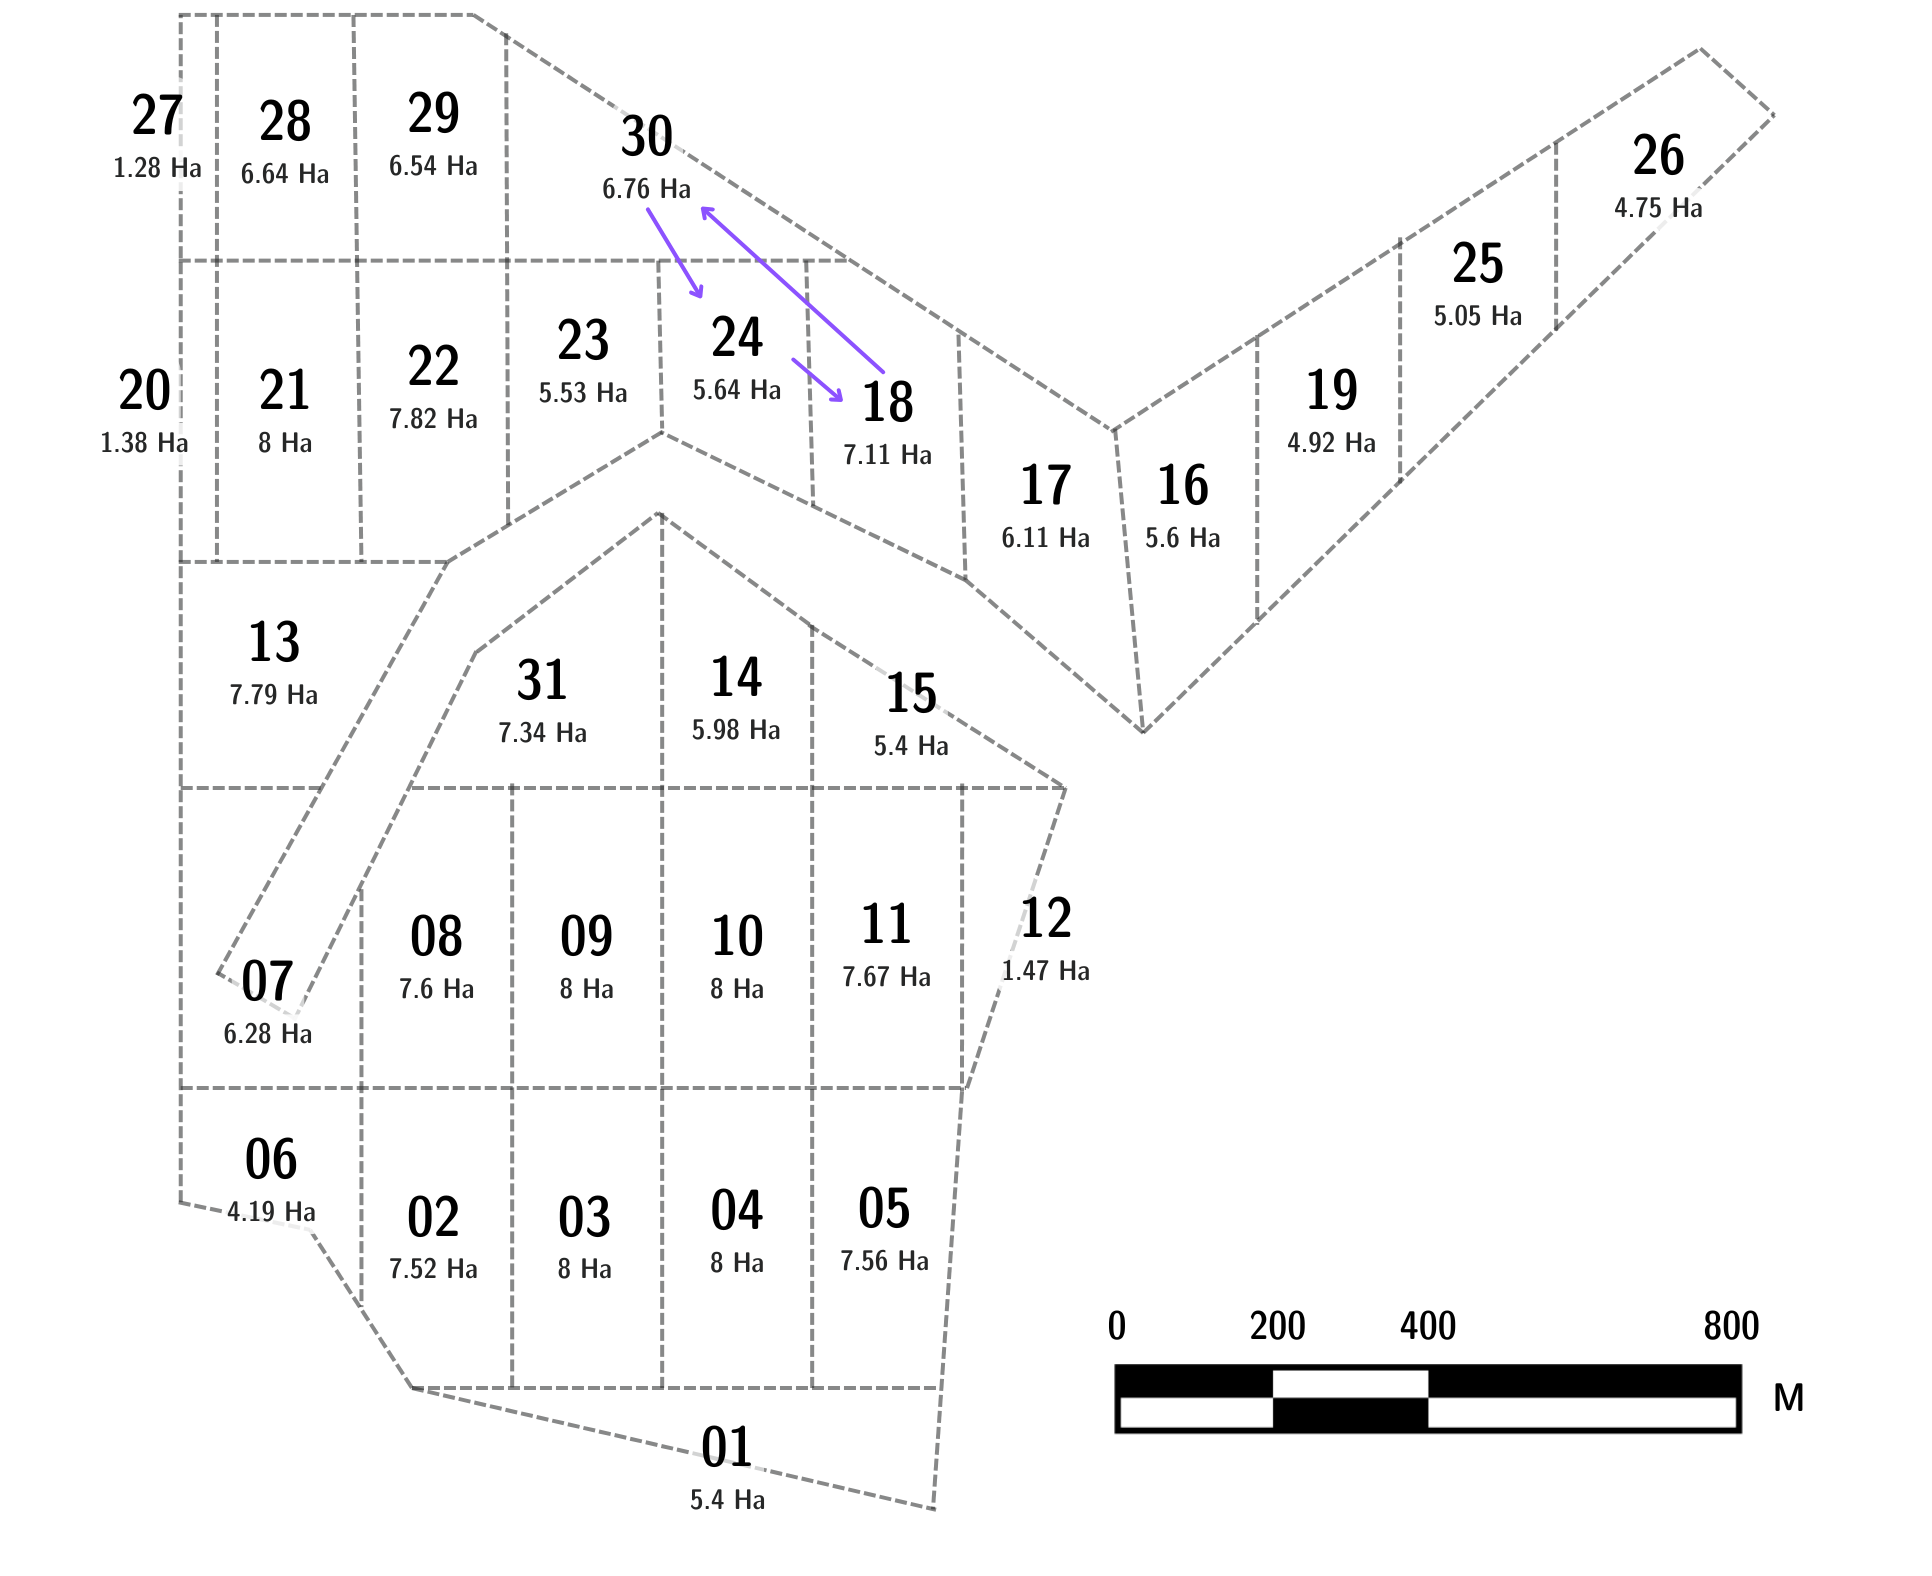
\includegraphics[width=0.40\linewidth]{Sources/Route13.png}
                }
                \caption{Some routes that are part of the heuristic solution.}
                \label{fig:RutasDeEjemplo}
            \end{center}
        \end{figure}
            
            For the integer part of the algorithm, 162.68 hours would be needed, while for the decimal part, 15.18 would be needed, hence, the result of the objective function is:
            
            $$z^* = 197.86 \text{ hours}$$

            Equivalent to 25 working days of 8 hours each if we consider only one vehicle, although this time can be improved if several vehicles operate simultaneously. It is important to mention that this solution requires 183 travels, just the estimated minimum estimated by the lower bound $\lceil \sum_{i} q_i \div L \rceil = 183$, showing its feasibility.
            
            Once the routes are ordered by the mathematical model proposed on Section \ref{OrderRoutes}, due to computing time limitations, we were only able to get a solution for 27 days, but the model got a possible minimum of 26 work days according to CPLEX, so we decided to do it by hand, which can be observed in Table \ref{tab:DistribucionViajes}.
            
            \begin{table}[!htp]\centering
            \scriptsize
            \begin{tabular}{lrrrrrr}\toprule
            \textbf{Day} &\textbf{Total Hours} &\textbf{Hours per Tour} &\textbf{Distributed load (Ha)} &\textbf{Tour} &\textbf{Iterations} \\\midrule
            1 &1.000 &1.000 & \{0.40, 0.56, 0.04\} &\{1 , 5, 11\} &1 \\
            1 &5.700 &1.140 & \{1\} & \{1\} &5 \\
            2 &7.790 &1.113 &\{1\} & \{5\} &7 \\
            3 &7.800 &1.114 &\{1\} &  \{4\} &7 \\
            4 &1.100 &1.100 &\{1\} &\{4\} &1 \\
            4 &6.670 &1.112 &\{1\} &\{3\} &6 \\
            5 &2.220 &1.110 &\{1\} &\{3\} &2 \\
            5 &5.367 &1.073 &\{1\} &\{10\} &5 \\
            6 &3.220 &1.073 &\{1\} &\{10\} &3 \\
            6 &4.320 &1.080 &\{1\} &\{9\} &4 \\
            7 &4.320 &1.080 &\{1\} &\{9\} &4 \\
            7 &1.000 &1.000 &\{0.19, 0.52, 0.29\} &\{6, 2, 8\} &1 \\
            7 &2.254 &1.127 &\{1\} &\{2\} &2 \\
            8 &5.636 &1.127 &\{1\} &\{2\} &5 \\
            8 &2.186 &1.093 &\{1\} &\{8\} &2 \\
            9 &5.464 &1.093 &\{1\} &\{8\} &5 \\
            9 &2.260 &1.130 &\{1\} &\{6\} &2 \\
            10 &2.260 &1.130 &\{1\} &\{6\} &2 \\
            10 &1.000 &1.000 &\{0.28, 0.31, 0.34, 0.07\} & \{7, 8, 14, 15\} &1 \\
            10 &4.440 &1.110 &\{1\} &\{7\} &4 \\
            11 &2.222 &1.111 &\{1\} &\{7\} &2 \\
            11 &5.267 &1.053 &\{1\} &\{14\} &5 \\
            11 &2.107 &1.053 &\{1\} &\{14\} &2 \\
            12 &1.000 &1.000 &\{0.75, 0.05, 0.2\} &\{26, 25, 19\} &1 \\
            12 &4.436 &1.109 &\{1\} &\{26\} &4 \\
            12 &2.169 &1.084 &\{1\} &\{25\} &2 \\
            13 &3.253 &1.084 &\{1\} &\{25\} &3 \\
            13 &4.250 &1.063 &\{1\} &\{19\} &4 \\
            14 &1.000 &1.000 &\{0.72, 0.28\} &\{19, 16\} &1 \\
            14 &5.230 &1.046 &\{1\} &\{16\} &5 \\
            14 &1.000 &1.000 &\{0.36, 0.11\} &\{16, 17\} &1 \\
            15 &3.060 &1.020 &\{1\} &\{17\} &3 \\
            15 &3.060 &1.020 &\{1\} &\{17\} &3 \\
            15 &1.000 &1.000 &\{0.63, 0.37\} &\{11, 12\} &1 \\
            16 &4.280 &1.070 &\{1\} &\{11\} &4 \\
            16 &3.220 &1.070 &\{1\} &\{11\} &3 \\
            17 &1.060 &1.060 &\{1\} &\{12\} &1 \\
            17 &1.000 &1.000 &\{0.10, 0.4, 0.5\} &\{12, 31, 15\} &1 \\
            17 &5.215 &1.043 &\{1\} &\{31 &\} \\
            18 &1.000 &1.000 &\{0.28, 0.64, 0.08\} &\{27, 28, 29\} &1 \\
            18 &1.100 &1.100 &\{1\} &\{27\} &1 \\
            18 &5.450 &1.090 &\{1\} &\{28\} &5 \\
            19 &1.090 &1.090 &\{1\} &\{28\} &1 \\
            19 &6.400 &1.067 &\{1\} &\{29\} &6 \\
            20 &1.000 &1.000 &\{0.46,0.54\} &\{29,30 &1\} \\
            20 &6.290 &1.048 &\{1\} &30 &6 \\
            21 &1.000 &1.000 &\{0.22, 0.34\} &\{30, 24\} &1 \\
            21 &5.104 &1.021 &\{1\} &\{24\} &5 \\
            21 &1.000 &1.000 &\{0.17, 0.53, 0.3\} &\{22, 23, 24\} &1 \\
            22 &4.163 &1.041 &\{1\} &\{23\} &4 \\
            22 &1.041 &1.041 &\{1\} &\{23\} &1 \\
            22 &1.000 &1.000 &\{0.38, 0.62\} &\{20, 22\} &1 \\
            22 &1.090 &1.090 &\{1\} &\{20\} &1 \\
            23 &5.400 &1.080 &\{1\} &\{21\} &5 \\ 
            23 &2.160 &1.080 &\{1\} &\{21\} &2 \\
            24 &7.400 &1.057 &\{1\} &\{22\} &7 \\
            25 &7.609 &1.087 &\{1\} &\{13\} &7 \\
            26 &1.000 &1.000 &\{0.97, 0.03\} &\{13, 22\} &1 \\
            26 &5.204 &1.041 &\{1\} &\{15\} &5 \\
            26 &1.000 &1.000 &\{0.41\} &\{15\} &1 \\
            \bottomrule
            \end{tabular}
            \vspace{10pt}
            \caption{Complete work plan for one truck.}\label{tab:DistribucionViajes}
        \end{table}
            
            
            
            
       
            \subsection{Software and Hardware Specifications}
            
            The experimentation for both the mathematical model and the heuristic model, was implemented on a computer with these characteristics.
    
            \begin{itemize}
                \item \textit{PC model:} Dell G15 5520
                \item \textit{Operative system:} Windows 11.
                \item \textit{Hard disk capacity:} 512GB
                \item \textit{RAM memory:} 16GB.
                \item \textit{Type of processor:} 12th Gen Intel(R) Core(TM)
                \item \textit{Number of cores:} 7
                \item \textit{Softwares:} For the mathematical model PuLP 2.8.0 in Python with the CPLEX license of IBM was used. For the heuristic model Pandas 2.2 in Python was used.
            \end{itemize}
            
            \subsection{Discussion}
    
    As expected in complex logistics problems, exact solution was highly computationally expensive, both in time and memory. As a result, a heuristic approach had to be implemented.
    
    It can be observed in table \ref{tab:TiemposDeComputo} that the mean GAP for all test cases is small enough to consider that the heuristic method provides solutions close to the optimum. It is important to keep in mind that five samples for each problem size are few to approximate the population mean for each size (which is not the objective of this experiment), hence, it should not be taken for granted that the relationship between them is especially significant. Even so, since this GAP is calculated on the entire problem (integer part plus decimal part), and the heuristic method is only applied on the decimal part, it is expected that the GAP will reduce as the problem size grows. This happens because the proportion of the solution cost that is associated with the integer part becomes larger as the problem grows, and the integer part is always optimized.
    
    Moreover, the results obtained by heuristics and the mathematical model for ordering the routes are congruent with the approximate time for the project given by the partnered entity, which expects to be able to complete the reforestation in less that a month, while in an ideal scenario, where no external issue affect the delivery times, the project could be completed in 26 days using the methodology described in this paper, successfully reducing the economic cost and time needed.


    
% -----------------------------Conclusion---------------------------------
    \section{Conclusions}
    Exact solutions based on the mathematical models permits to find the best possible way to solve a problem, which is translated to a considerable reduction of cost. However, there are some cases, like the one presented in this paper, where finding these solutions becomes inconveniently large in terms of time and memory, at least for most of the commercial computers. This is when heuristics gain relevance, since finding solutions almost as good as the optimal with much less time and memory needed, is definitely an option to take in count for small projects and/or companies.

    Additionally, some possible future improvements for this project are listed.
    
    \begin{itemize}
        \item Integrating realistic distance metrics accounting for terrain and obstacles.
        \item Consider, tentatively with a statistical approach, those native specimens already found in the areas to be reforested and that do not need to be planted.
        \item Consider the effects of climatic phenomena on the execution of the logistics plan.
    \end{itemize}
    
    Finally, we provide a link to a \underline{\href{https://github.com/JuanjoBelt/VRP-ReforestationTransportLogistics}{GitHub repository}} containing all the implementations of the solution methods mentioned in this article, as well as all the information necessary to study and replicate it.


% -------------------------------------- REFERENCES --------------------------------------
    %\vspace{1cm}
    %\newpage
    \section{References}
    \printbibliography[title={References}, heading=none]

    
 \end{document}
